\begin{frame}
        \begin{block}{Stille Annahmen und Beschränkungen}
                \begin{itemize}
                        \pause \item Ein Zugriff ist nie Größer als eine Cachezeile
                               \item Ein Zugriff fällt nie in mehr als zwei Cachezeilen
                        \pause \item Alle Elemente einer Matrix sind gleich groß
                        \pause \item Nachbarn in einer Zeile der Matrix liegen im Speicher nebeneinander, übereinanderliegende Zeilen liegen im Speicher nebeneinander
                \end{itemize}
        \end{block}
\end{frame}

\subsection{Eventverarbeitungsstruktur} The GUI is implemented solely in Java, utilizing the Swing Architecture. The project is structured according to the Model–View–Controller pattern. It consists of three packages (\texttt{data}, \texttt{view} and \texttt{controller}), separating the data from the interface, connected through the \texttt{controller}. The package \texttt{data} is responsible for reading the data files and providing a comprehensive interface to retrieve the data. The package \texttt{view} is responsible for displaying the data to the user. It communicates with the data only via the \texttt{controller} (and vice versa). Therefore the \texttt{controller}'s purpose is to manage the entire data flow of the software. It sends requested data to the user interface or requests new data to be loaded from a file. 

\subsection{Class Responsibilities - Package \texttt{view}}
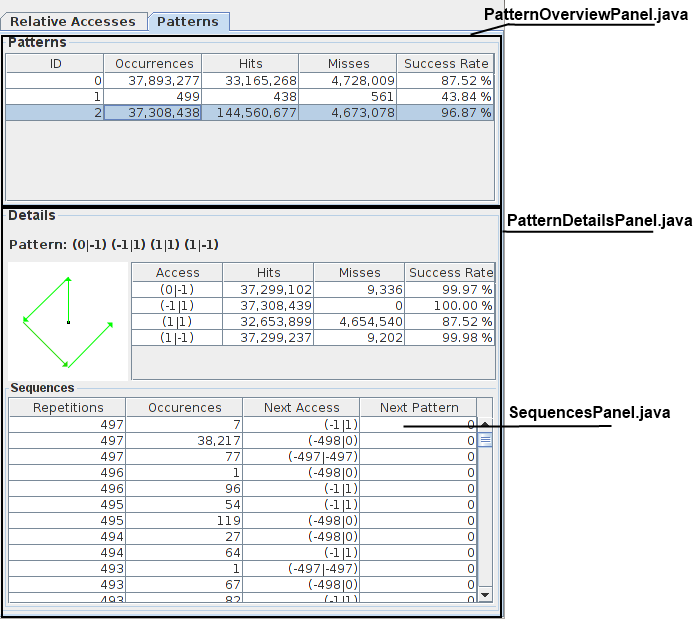
\includegraphics[width=350px]{gui/classresp2.png}
\newpage 
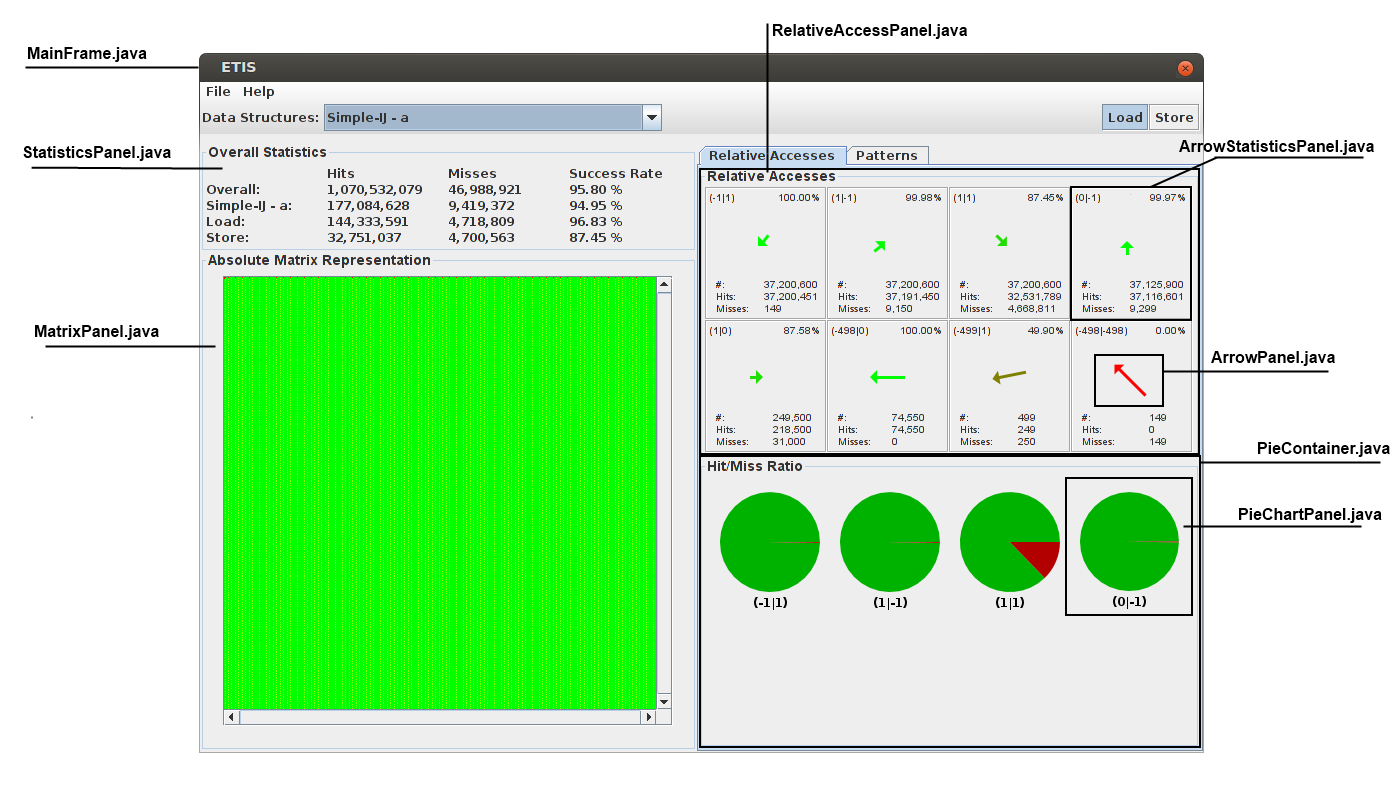
\includegraphics[angle=90,height=700px]{gui/classresp1.png}
\subsection{Informal Class Diagramm}
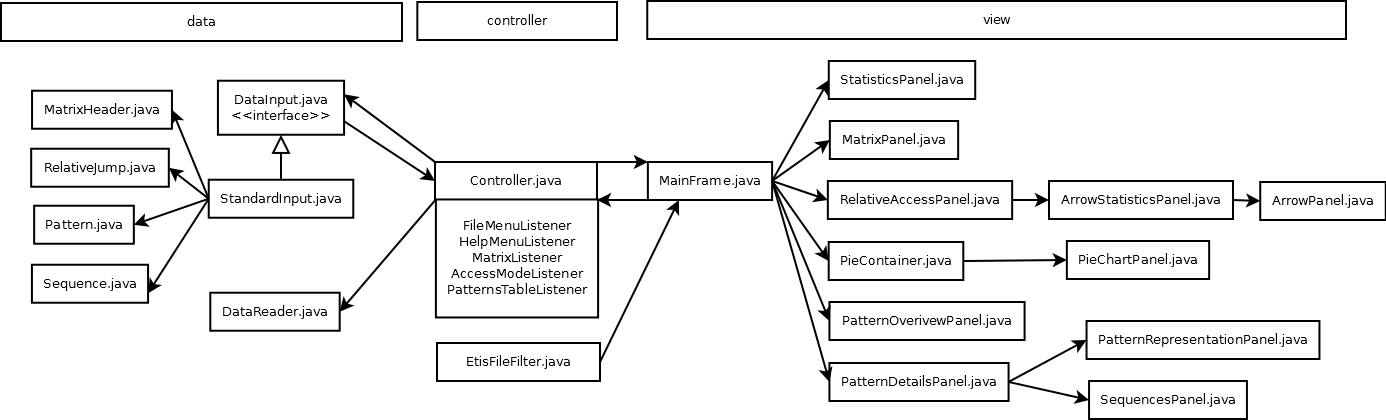
\includegraphics[angle=90,height=560px]{gui/comm.png} 
